% Options for packages loaded elsewhere
\PassOptionsToPackage{unicode}{hyperref}
\PassOptionsToPackage{hyphens}{url}
%
\documentclass[
  12pt,
]{article}
\usepackage{lmodern}
\usepackage{amssymb,amsmath}
\usepackage{ifxetex,ifluatex}
\ifnum 0\ifxetex 1\fi\ifluatex 1\fi=0 % if pdftex
  \usepackage[T1]{fontenc}
  \usepackage[utf8]{inputenc}
  \usepackage{textcomp} % provide euro and other symbols
\else % if luatex or xetex
  \usepackage{unicode-math}
  \defaultfontfeatures{Scale=MatchLowercase}
  \defaultfontfeatures[\rmfamily]{Ligatures=TeX,Scale=1}
\fi
% Use upquote if available, for straight quotes in verbatim environments
\IfFileExists{upquote.sty}{\usepackage{upquote}}{}
\IfFileExists{microtype.sty}{% use microtype if available
  \usepackage[]{microtype}
  \UseMicrotypeSet[protrusion]{basicmath} % disable protrusion for tt fonts
}{}
\makeatletter
\@ifundefined{KOMAClassName}{% if non-KOMA class
  \IfFileExists{parskip.sty}{%
    \usepackage{parskip}
  }{% else
    \setlength{\parindent}{0pt}
    \setlength{\parskip}{6pt plus 2pt minus 1pt}}
}{% if KOMA class
  \KOMAoptions{parskip=half}}
\makeatother
\usepackage{xcolor}
\IfFileExists{xurl.sty}{\usepackage{xurl}}{} % add URL line breaks if available
\IfFileExists{bookmark.sty}{\usepackage{bookmark}}{\usepackage{hyperref}}
\hypersetup{
  hidelinks,
  pdfcreator={LaTeX via pandoc}}
\urlstyle{same} % disable monospaced font for URLs
\usepackage{graphicx}
\makeatletter
\def\maxwidth{\ifdim\Gin@nat@width>\linewidth\linewidth\else\Gin@nat@width\fi}
\def\maxheight{\ifdim\Gin@nat@height>\textheight\textheight\else\Gin@nat@height\fi}
\makeatother
% Scale images if necessary, so that they will not overflow the page
% margins by default, and it is still possible to overwrite the defaults
% using explicit options in \includegraphics[width, height, ...]{}
\setkeys{Gin}{width=\maxwidth,height=\maxheight,keepaspectratio}
% Set default figure placement to htbp
\makeatletter
\def\fps@figure{htbp}
\makeatother
\setlength{\emergencystretch}{3em} % prevent overfull lines
\providecommand{\tightlist}{%
  \setlength{\itemsep}{0pt}\setlength{\parskip}{0pt}}
\setcounter{secnumdepth}{-\maxdimen} % remove section numbering

\author{}
\date{}

\begin{document}

Devoir n°6 : Routage - Rattrapage

On considère un réseau composé de plusieurs routeurs reliés de la façon
suivante :

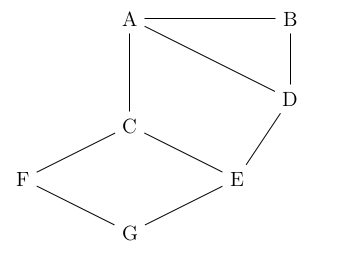
\includegraphics{data_sujet_0/sujet0_routage1.png}\{:.center\}

\hypertarget{le-protocole-rip}{%
\subsubsection{➡ Le protocole RIP}\label{le-protocole-rip}}

Le protocole RIP permet de construire les tables de routage des
différents routeurs, en indiquant pour chaque routeur la distance, en
nombre de sauts, qui le sépare d'un autre routeur. Pour le réseau
ci-dessus, on dispose des tables de routage suivantes :

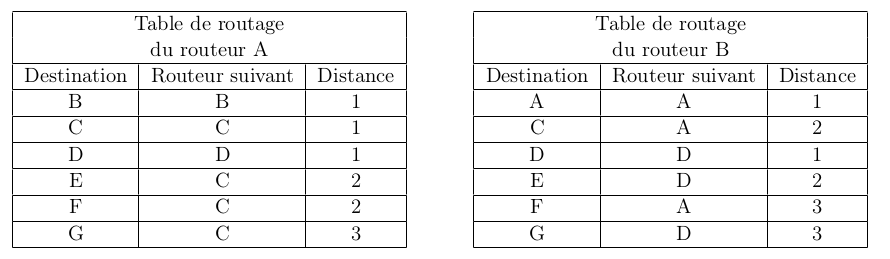
\includegraphics{data_sujet_0/sujet0_table1.png}\{:.center\}

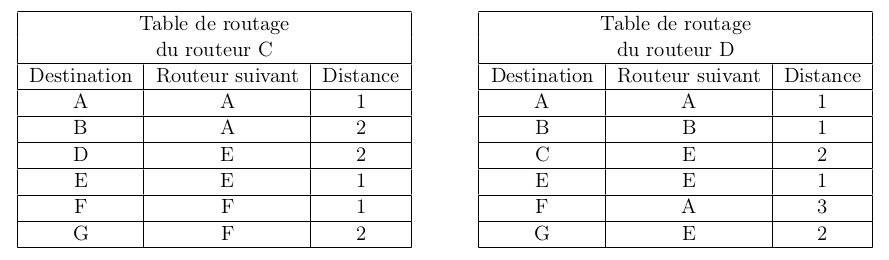
\includegraphics{data_sujet_0/sujet0_table2.png}\{:.center\}

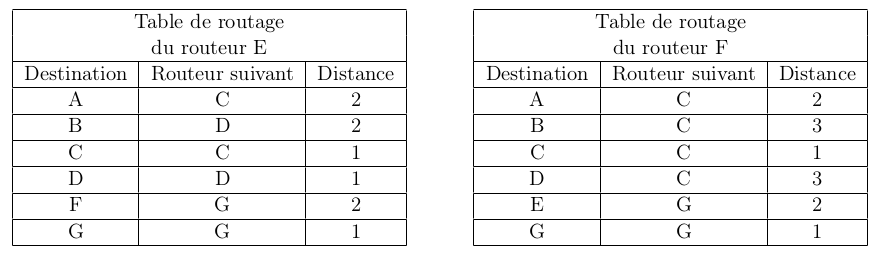
\includegraphics{data_sujet_0/sujet0_table3.png}\{:.center\}

!!! fabquestion ``Question 1'' 1. Le routeur A doit transmettre un
message au routeur G, en effectuant un nombre minimal de sauts.
Déterminer le trajet parcouru.\\
2. Déterminer une table de routage possible pour le routeur G obtenu à
l'aide du protocole RIP.

!!! fabquestion ``Question 2'' Le routeur C tombe en panne. Reconstruire
la table de routage du routeur A en suivant le protocole RIP.

\hypertarget{le-protocole-ospf}{%
\subsubsection{➡ Le protocole OSPF}\label{le-protocole-ospf}}

Contrairement au protocole RIP, l'objectif n'est plus de minimiser le
nombre de routeurs traversés par un paquet. La notion de distance
utilisée dans le protocole OSPF est uniquement liée aux coûts des
liaisons.\\
L'objectif est alors de minimiser la somme des coûts des liaisons
traversées.\\
Le coût d'une liaison est donné par la formule suivante :

\(coût = \dfrac{10^8}{d}\)

où \(d\) est la bande passante en bits/s entre les deux routeurs.

On a rajouté sur le graphe représentant le réseau précédent les
différents débits des liaisons.\\
On rappelle que 1 Gb/s = 1 000 Mb/s = \(10^9\) bits/s.

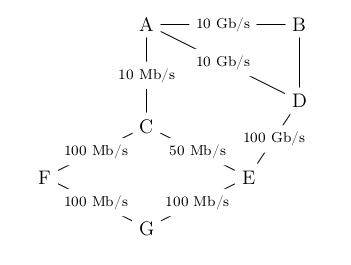
\includegraphics{data_sujet_0/ex5.png}\{:.center\}

!!! fabquestion ``Question 3'' 1. Vérifier que le coût de la liaison
entre les routeurs A et B est 0,01. 2. La liaison entre le routeur B et
D a un coût de 5. Quel est le débit de cette liaison ?

!!! fabquestion ``Question 4'' Le routeur A doit transmettre un message
au routeur G, en empruntant le chemin dont la somme des coûts sera la
plus petite possible. Déterminer le chemin parcouru. On indiquera le
raisonnement utilisé.

\end{document}
